\exercise

Describe the randomized algorithm for I/O-efficiently extract an independent set
from a list.

\solution

For each item in the list we toss a (fair) coin, and then we select those items
$i$ such that $coin(i) = \text{\tt H}$ (head) and $coin(succ(i)) = \text{\tt T}$
(tail). There is no chance that, for any $i$, both $i$ and $succ(i)$ will be
selected, so the resulting set of item will be an independent set\footnote{This
holds also if we choose the configuration {\tt TH} instead of {\tt HT}, while it
would not work for {\tt HH} or {\tt TT}, since the same face of the coin may
come three or more consecutive times, causing two or more consecutive items to
be selected, thus producing a non-independent set.}. The probability that an
item is selected is $1/4$, since we chose only one of 4 possible 2-coins
configurations. So the average number of selected items will be $n/4$. It can be
proved that the size of the set will be strongly concentrated around this value,
so we may want to repeat the coin tossing until the resulting size will be
greater or equal than $n/c$, for some $c > 4$. In the 2-levels memory model,
this can be done as follows: given a list $\mathcal{L}$, we store in memory a
quadruple for each of its items, in the form of $\langle i, succ(i), \text{\tt
\_}, \text{\tt \_} \rangle$, where the third and fourth elements are
placeholders for the values of $coin(i)$ and $coin(succ(i))$. Then we perform
the selection using a random coin-tossing and a sequence of {\tt sort} and {\tt
scan} primitives. Taking for example the list in \autoref{fig:coin-tossing}, we
first toss a coin for each item of the list and then we select the independent
set as follows:
%
\begin{align*}
  \begin{matrix}
    \langle 1, 6, \text{\tt H}, \text{\tt \_} \rangle \\
    \langle 2, 7, \text{\tt H}, \text{\tt \_} \rangle \\
    \langle 3, 5, \text{\tt T}, \text{\tt \_} \rangle \\
    \langle 4, 2, \text{\tt T}, \text{\tt \_} \rangle \\
    \langle 5, 8, \text{\tt H}, \text{\tt \_} \rangle \\
    \langle 6, 6, \text{\tt H}, \text{\tt \_} \rangle \\
    \langle 7, 3, \text{\tt T}, \text{\tt \_} \rangle \\
    \langle 8, 1, \text{\tt T}, \text{\tt \_} \rangle \\
  \end{matrix}
  \stackrel{\text{\tiny \tt sort}}{\longmapsto}
  \begin{matrix}
    \langle 8, 1, \text{\tt T}, \text{\tt \_} \rangle \\
    \langle 4, 2, \text{\tt T}, \text{\tt \_} \rangle \\
    \langle 7, 3, \text{\tt T}, \text{\tt \_} \rangle \\
    \langle 3, 5, \text{\tt T}, \text{\tt \_} \rangle \\
    \langle 1, 6, \text{\tt H}, \text{\tt \_} \rangle \\
    \langle 6, 6, \text{\tt H}, \text{\tt \_} \rangle \\
    \langle 2, 7, \text{\tt H}, \text{\tt \_} \rangle \\
    \langle 5, 8, \text{\tt H}, \text{\tt \_} \rangle \\
  \end{matrix}
  \stackrel{\text{\tiny \tt scan}}{\longmapsto}
  \begin{matrix}
    \langle 8, 1, \text{\tt T}, \text{\tt H} \rangle \\
    \langle 4, 2, \text{\tt T}, \text{\tt H} \rangle \\
    \langle 7, 3, \text{\tt T}, \text{\tt T} \rangle \\
    \langle 3, 5, \text{\tt T}, \text{\tt H} \rangle \\
    \langle 1, 6, \text{\tt H}, \text{\tt H} \rangle \\
    \langle 6, 6, \text{\tt H}, \text{\tt H} \rangle \\
    \langle 2, 7, \text{\tt H}, \text{\tt T} \rangle \\
    \langle 5, 8, \text{\tt H}, \text{\tt T} \rangle \\
  \end{matrix}
  \stackrel{\text{\tiny \tt sort}}{\longmapsto}
  \begin{matrix}
    \langle 1, 6, \text{\tt H}, \text{\tt H} \rangle \\
    \langle 2, 7, \text{\tt H}, \text{\tt T} \rangle \\
    \langle 3, 5, \text{\tt T}, \text{\tt H} \rangle \\
    \langle 4, 2, \text{\tt T}, \text{\tt H} \rangle \\
    \langle 5, 8, \text{\tt H}, \text{\tt T} \rangle \\
    \langle 6, 6, \text{\tt H}, \text{\tt H} \rangle \\
    \langle 7, 3, \text{\tt T}, \text{\tt T} \rangle \\
    \langle 8, 1, \text{\tt T}, \text{\tt H} \rangle \\
  \end{matrix}
  \stackrel{\text{\tiny \tt scan}}{\longmapsto}
  \begin{matrix}
    \langle 1, 6, \text{\tt H}, \text{\tt H} \rangle \phantom{\longrightarrow \text{\bf select}\ 2\ }\\
    \langle 2, 7, \underline{\text{\tt H}, \text{\tt T}} \rangle \longrightarrow \text{\bf select}\ 2\\
    \langle 3, 5, \text{\tt T}, \text{\tt H} \rangle \phantom{\longrightarrow \text{\bf select}\ 2\ }\\
    \langle 4, 2, \text{\tt T}, \text{\tt H} \rangle \phantom{\longrightarrow \text{\bf select}\ 2\ }\\
    \langle 5, 8, \underline{\text{\tt H}, \text{\tt T}} \rangle \longrightarrow \text{\bf select}\ 5\\
    \langle 6, 6, \text{\tt H}, \text{\tt H} \rangle \phantom{\longrightarrow \text{\bf select}\ 2\ }\\
    \langle 7, 3, \text{\tt T}, \text{\tt T} \rangle \phantom{\longrightarrow \text{\bf select}\ 2\ }\\
    \langle 8, 1, \text{\tt T}, \text{\tt H} \rangle \phantom{\longrightarrow \text{\bf select}\ 2\ }\\
  \end{matrix}
\end{align*}
%
\begin{figure}[H]
  \centering
  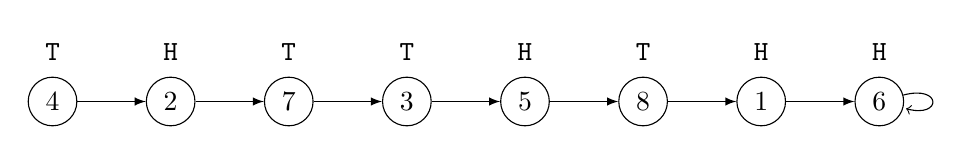
\begin{tikzpicture}[node distance=1.5cm, every node/.append style={draw,circle}]
    \node[label={\tt T}] (a) {4};
    \node[right of=a, label={\tt H}] (b) {2};
    \node[right of=b, label={\tt T}] (c) {7};
    \node[right of=c, label={\tt T}] (d) {3};
    \node[right of=d, label={\tt H}] (e) {5};
    \node[right of=e, label={\tt T}] (f) {8};
    \node[right of=f, label={\tt H}] (g) {1};
    \node[right of=g, label={\tt H}] (h) {6};
    \draw[-latex] (a) -- (b);
    \draw[-latex] (b) -- (c);
    \draw[-latex] (c) -- (d);
    \draw[-latex] (d) -- (e);
    \draw[-latex] (e) -- (f);
    \draw[-latex] (f) -- (g);
    \draw[-latex] (g) -- (h);
    \path (h) edge[-latex, loop right] (h);
  \end{tikzpicture}
  \caption{List of items with their respective coin-tossing results.}
  \label{fig:coin-tossing}
\end{figure}
